\section{Data Analysis}
\label{sec:analysis}

The analysis lives in \code{notebooks/01\_eda.ipynb}, and every statistic below is written to
\code{eda\_tests.csv}. Each finding is stated as an observation, the statistic behind it, and the decision it
informed.

\textbf{Finding 1: the features are heavy-tailed.} Amounts, gaps and ratios span several orders of magnitude
(Figure~\ref{fig:distributions}). The raw amount has a skewness of \V{eda.f1_skew_raw}, but only
\V{eda.f1_skew_log} on a logarithmic scale; the size ratio's excess kurtosis is \V{eda.f4_kurt_raw}. A mean and
standard deviation would be dominated by a few extreme values, so we compare on log scales and use the median
and median absolute deviation.

\begin{figure}[ht]
\centering
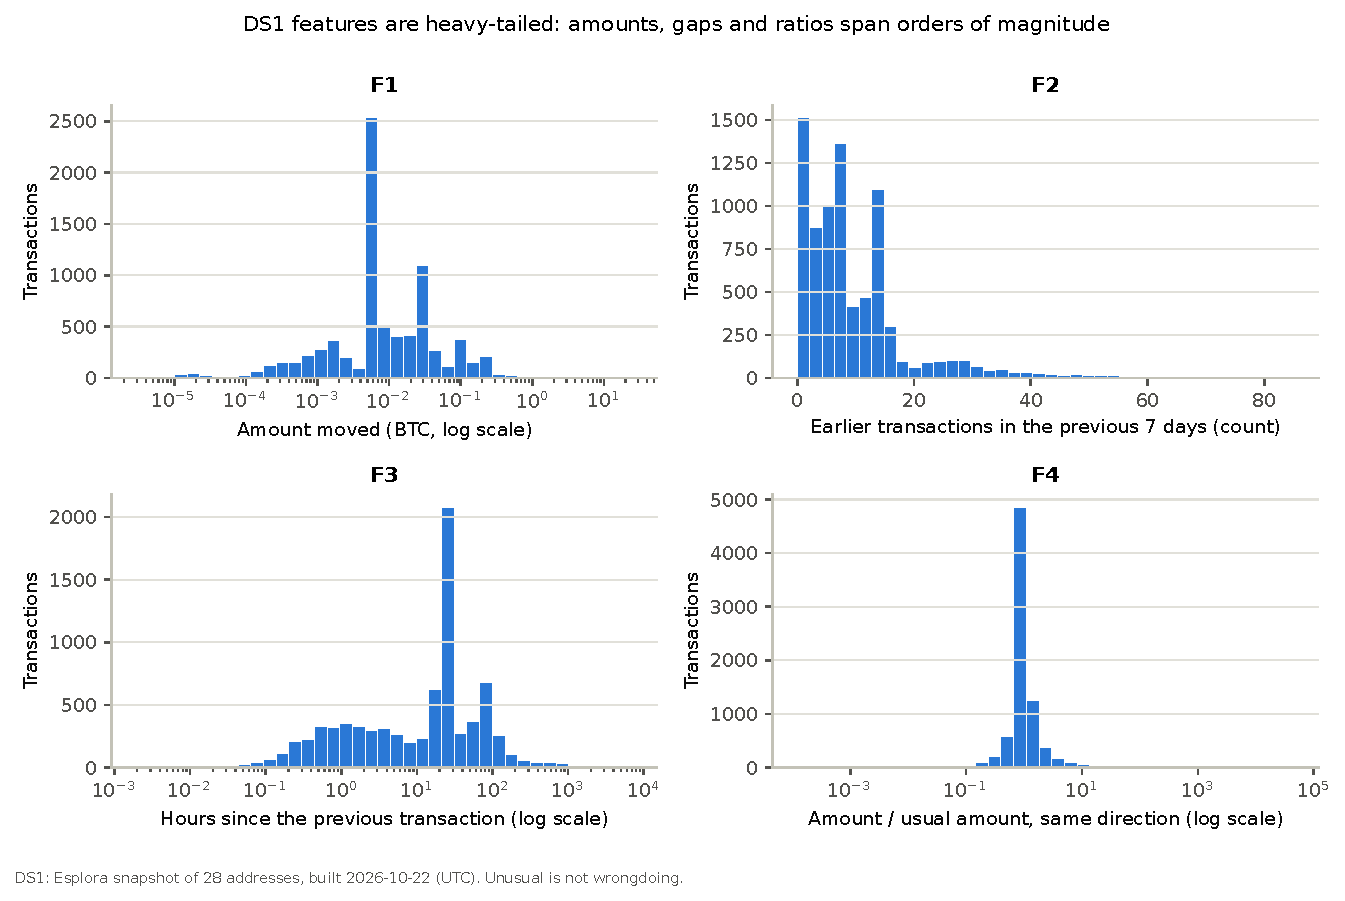
\includegraphics[width=0.82\textwidth]{eda_feature_distributions.pdf}
\caption{DS1's four features. Amounts (F1), gaps (F3) and size ratios (F4) span orders of magnitude, which is why
they are compared on log scales with robust statistics.}
\label{fig:distributions}
\end{figure}

\textbf{Finding 2: every address has its own scale.} The median amounts of DS1's main addresses differ by a
factor of \V{eda.scale_ratio}, and for \V{eda.dir_differ} of the \V{eda.dir_tested} addresses with enough
transactions in both directions, received and sent amounts differ (Mann--Whitney U, $p<0.05$;
Figure~\ref{fig:direction}). One global threshold cannot fit every address, so each feature is compared with the
same address's history and amounts only with earlier transactions in the same direction. The ablation confirms
the decision: A1's original definition, without these refinements, flags \V{abl.written_flag_rate} of real
transactions with a mean planted recall of \V{abl.written_recall}, against \V{abl.refined_flag_rate} and
\V{abl.refined_recall} for the refined features (\code{eval\_ablation.csv}).

\begin{figure}[ht]
\centering
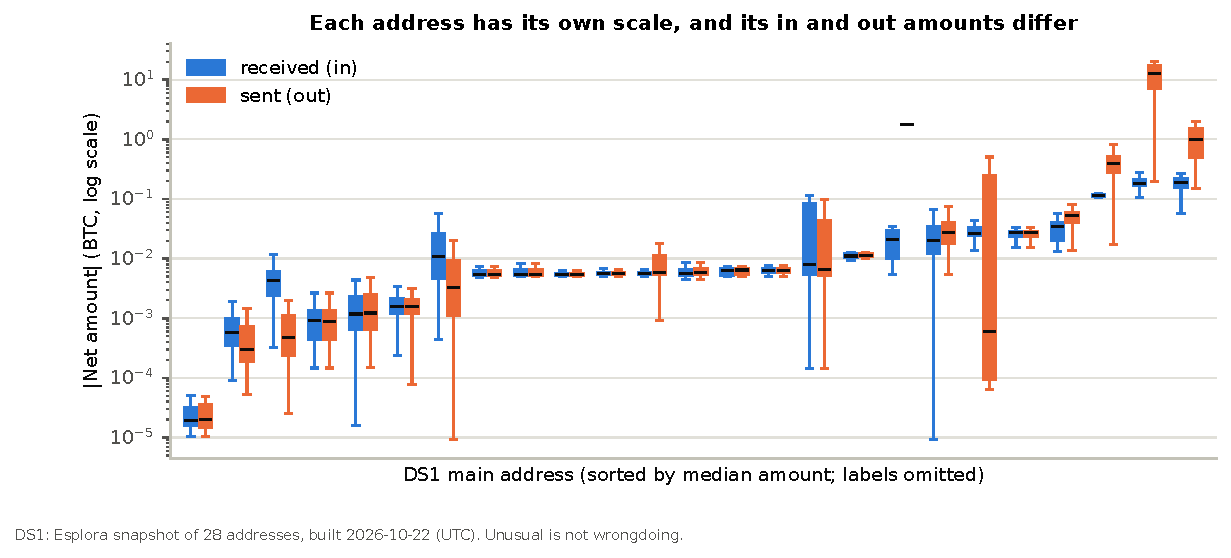
\includegraphics[width=0.9\textwidth]{eda_direction_amounts.pdf}
\caption{Received and sent amounts per DS1 main address (box: quartiles; line: median). Scales differ by four
orders of magnitude, and many addresses send amounts unlike those they receive.}
\label{fig:direction}
\end{figure}

\textbf{Finding 3: labels are rare and drift over time.} Elliptic's illicit share among labelled transactions is
\V{eda.ell_train_share} in the training steps but \V{eda.ell_test_share} in the test steps, and
\V{eda.ell_unknown} of all rows are unlabelled. BitcoinHeist's positives are \V{eda.heist_share} of rows, and
every feature separates them only weakly (largest rank-biserial effect \V{eda.heist_max_effect}). Accuracy
would reward predicting the majority class (Chicco and Jurman 2020), so we split by time, report precision,
recall, F1 and the area under the precision--recall curve (PR-AUC), and include class weights in tuning. The weak
BitcoinHeist effects also anticipated its poor classification results in Section~\ref{sec:evaluation}.
